\documentclass[10pt]{article}

\usepackage{footnote}
\usepackage{url}
\usepackage{wrapfig}
\usepackage{subfig}
\usepackage{graphicx}
\usepackage{hyperref}
\usepackage[hmargin=3cm,vmargin=3.5cm]{geometry}
\title{Linear Logic and Coordination for Parallel Programming}

\author{Flavio Cruz \href{mailto:fmfernan@cs.cmu.edu}{(fmfernan@cs.cmu.edu)} \\\\
\textbf{Committee}: \\
Umut Acar\\
Luis Barbosa\\
Seth Goldstein\\
Carlos Guestrin\\
Frank Pfenning\\
Ricardo Rocha\\
}

\begin{document}

\maketitle

The purpose of this document is to clarify and re-state the thesis statement
presented in the old proposal document~\footnote{Available in
\url{http://www.andrew.cmu.edu/user/fmfernan/proposal.pdf}}.
In a nutshell, the thesis statement has changed from focusing on implementing the
language efficiently to make programs more scalable. We also focus on proving that programs
are correct and that adding coordination directives does not
make the program incorrect but only provide better execution behavior (faster,
      less memory usage, more scalable).
We finally discuss the latest work done to accomplish the new thesis goals.

\section{Thesis Statement}

We propose Linear Meld (LM), a new linear logic programming language, designed
to write parallel graph based programs on multicores.  We argue that LM is a
superior declarative programming model because it not only automatically
parallelizes programs, but, in cases where it is necessary, it allows the
programmer to control parallel scheduling and placement of data to further
improve the program run time and scalability.  Since LM is based on solid
logical foundations, we argue that we can also prove interesting properties of
programs, including correctness and termination. We will prove our thesis
through five major goals:

\begin{itemize}
   
   \item Linear Logic (mostly done)

   We integrated linear logic into our language, so that program state can be
   encoded naturally. The original Meld was fully based on classical logic where
   everything that is derived is true forever. Linear logic turns some facts
   into resources that will be consumed when a rule is applied.  To the best of
   our knowledge, LM is the first linear logic based language implementation
   that attempts to solve real world problems.

   \item Coordination (partly done)
   
   LM offers execution control to the programmer through the use of coordination
   directives to make the program faster and more scalable. These coordination
   directives change how the runtime system schedules computation and can be
   written with the same facilities used to write standard program code.  We are
   using the concept of \emph{action facts} to coordinate the execution of
   programs.  We can increase the priority of certain nodes during runtime
   according to the state of the computation and to the state of the runtime in
   order to make better scheduling decisions so that programs can run faster.
   We intend to add more coordination directives and action facts and also write
   more programs that can take advantage of coordination.
   
   \item Provability (partly done)
   
   Since LM is a logic programming language, we want to leverage the logical
   foundations of the language to show how to prove properties of a few
   programs. We are mostly interested in proving correctness and termination.
   We also want to show that coordination directives do not change those
   correctness proofs of programs but only improve run time, scalability or
   memory usage.

   \item Multicore Parallelism (partly done)
   
   We divide the logical facts across all the nodes of the graph. Since the
   logical rules only make use of facts from a node, computation can be
   performed locally, without reference from other nodes of the graph.
   We envision the application as a communicating graph data structure where
   each processing unit performs work on a different subset of the graph, thus
   enabling concurrency. This is an advantage of LM since we can run programs on
   many different types of distributed systems as long as the underlying runtime
   system uses the appropriate communication facilities.

   \item Experimental Results (partly done)

   We have implemented a new compiler and a virtual machine prototype from
   scratch that executes on multicore machines.  We have implemented programs
   such as belief propagation, belief propagation with residual splash,
   PageRank, graph coloring, N queens, shortest path, diameter estimation,
   MapReduce, game of life, quick-sort, neural network training, among others.
   Our preliminary results show that our particular implementation provides
   good scalability with at least 16 threads.
   
\end{itemize}

\section{Road Map}

The thesis roadmap has three major goals.

\subsection{First Major Goal: Improved Coordination Mechanisms and Programs}

The LM runtime is able to scale programs reasonably well in multicore
architectures. The use of coordination directives further improves the execution
time, scalability and memory use of programs by allowing the programmer to
fine tune them with sensing and action facts.
However, there's still some scalability issues in our implementation that reduce the applicability of
coordination when dealing with coordination information that must be
exchanged between threads. Our first major goal is thus to improve
the efficiency of coordination directives and associated coordination code.

We want to implement more programs that use coordination in order to find out
which new coordination facts may be appropriate in our system. We are specially
interested in designing more sensing and action facts that place nodes in
specific threads to improve data locality.  For instance, some multicore
architectures employ a cache hierarchy where cores are clustered, therefore some
pairs of clusters will communicate faster. It might be a good idea to give the
programmer access to the graph of processing units or allow a processing unit to
be placed on certain cores in order to improve computation time.

A potential algorithm that we can implement is the Alpha-Beta search algorithm,
since we are able to reduce the search space by prioritizing certain tree branches.
However, it remains to be seen if the program can be easily implemented in LM.
We intend to measure the execution speedup of these new coordinated programs.

\subsection{Second Major Goal: Improved General Scalability}

Our second goal is to improve the overall scalability of the system, specially
when using more than 16 threads. To accomplish this, we first need to understand
how threads communicate, specially in terms of node stealing and load balancing.
For instance, our simple node stealing algorithm needs to be revamped in order
to use better stealing heuristics such as stealing nodes that are closer (in
terms of connections) to the thread's set of owned nodes.

\subsection{Third Major Goal: Proofs of Interesting Program Properties}


We want to take a few programs and prove their correctness and
termination using informal proofs based on the operational semantics of the
language. Good candidates include the shortest distance algorithm, the
quick-sort algorithm, the minimax algorithm and the heat transfer algorithm.
These proofs will provide examples and techniques for future formalization, which
is beyond the scope of the thesis. We are also interested in proving that
adding coordination directives to some of these programs does not change their
correctness proofs and only improve the convergence time or scalability.

\section{New Developments}

In the current semester, we have been working towards the three major goals.

\subsection{Improved Coordination Mechanisms and Programs}

We have specified new coordination directives that allows us to further
optimize scalability, memory usage and runtime of our programs. We added the
following action facts to our language:

\begin{description}
   \item[set-cpu(A, P)]: Place node \texttt{A} in thread \texttt{P}. Node
   \texttt{A} can no longer be moved to another thread.
   \item[set-affinity(A, B)]: Place node \texttt{A} in the same thread where
   \texttt{B} is currently located.
   \item[set-static(A)]: Do not allow node \texttt{A} to be moved to another
   thread.
   \item[set-moving(A)]: Allow node \texttt{A} to be moved around.
   \item[set-default-priority(A, P)]: Set the default priority of node
   \texttt{A} to \texttt{P}. The priority is always used whenever the node is to
   be scheduled for further derivations.
\end{description}

As we have seen, most of the new directives (except the last one) deal with node
partitioning and affinity. This a nice addition to our language since most
coordination directives we already had were related to computation scheduling.

We have been experimenting with the new coordination directives and we have been
exploring programs that may benefit from them. One good example is the MiniMax
program shown in Fig.~\ref{fig:coord}. We coordinated the program so that deeper
nodes have a higher priority than the nodes closer to the root of the tree. This
forces the virtual machine to expand the search tree using a depth-first
approach, thus reducing the size of the tree that needs to be kept in memory. We
have seen a huge reduction in terms of memory usage: the original version used
around 13GB of memory, while the coordinated version uses only a few MBs. We
also fine tuned parallel execution by forcing deeper nodes to be kept in the
same thread, improving memory locality. These new coordination directives allows
us to improve scalability, as it can be seen from Fig.~\ref{fig:coord}.

%\begin{wrapfigure}[20]{L}{0.45\textwidth}
\begin{figure}[ht]
  \begin{center}
   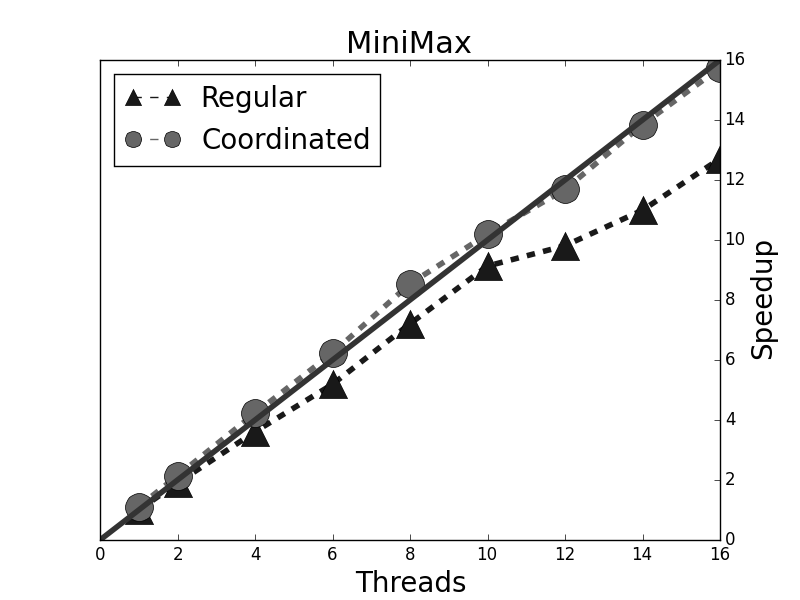
\includegraphics[width=0.45\textwidth]{figures/coord_min-max-tictactoe}
\end{center}
\caption{Scalability and performance gains by using coordination in the MiniMax
   program. The speedup of the regular and coordinated version is calculated
   from the sequential execution time of the regular version. The coordinated
   version with 16 threads is 16 times faster than the regular version without
   coordination using a single thread.}
\label{fig:coord}
\end{figure}

We have experimented with node partitioning in the N Queens program and
so far the results indicate that, without work stealing, coordination directives
such as \texttt{set-cpu} improve performance by a factor of two. We have
yet to see if such directives allows us significant improvements in the presence
of work stealing.

In terms of implementation, we have improved sharing of coordination
information between threads. While previous results showed that
coordinated programs would perform worse when using coordination, we now see
that they perform better when using multiple threads. Our preliminary
results are shown in Fig.~\ref{fig:coord_others}.

\begin{figure*}[hb]
\begin{center}
  \subfloat[]{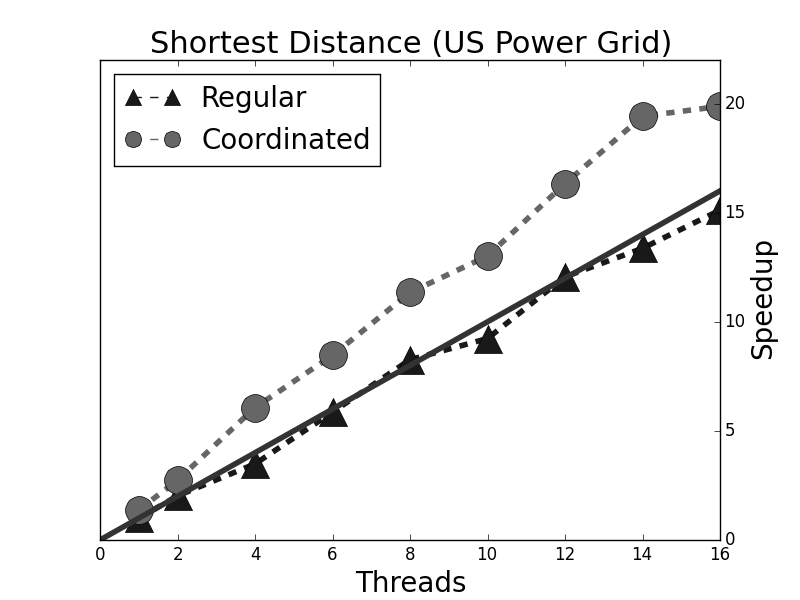
\includegraphics[width=0.35\textwidth]{figures/coord_shortest-uspowergrid}}
  \subfloat[]{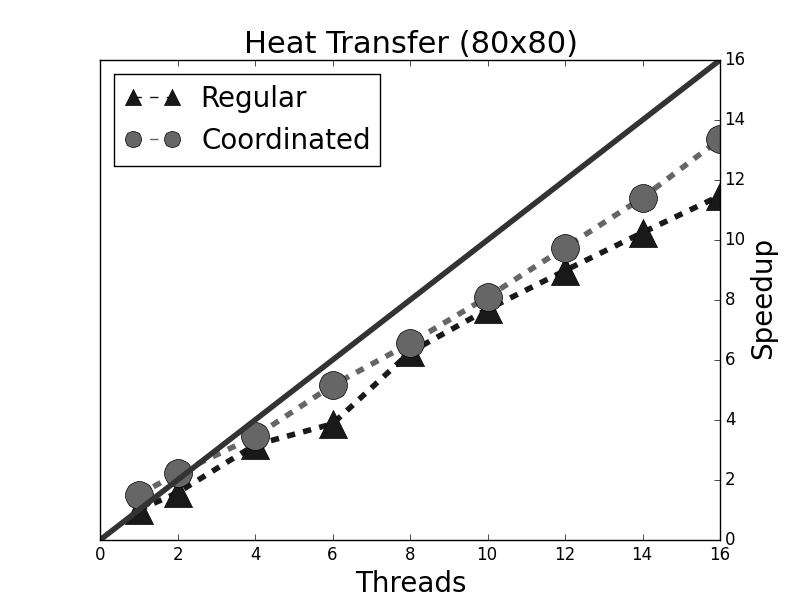
\includegraphics[width=0.35\textwidth]{figures/coord_new-heat-transfer-80}}
\end{center}
\caption{Scalability and performance gains by using coordination in the Shortest
Distance and Heat Transfer programs. We have changed our implementation so that
coordination information is exchanged between threads, thus enabling
continued performance improvements even when using many threads.}
\label{fig:coord_others}
\end{figure*}

\subsection{Improved General Scalability}

In order to improve the scalability of our runtime, we made several adjustments
to the virtual machine. Most of the performance enhancements deal with improved
memory organization, less thread communication, improved work stealing, improved
locks and elimination of sequential bottlenecks. We compared the scalability of the
improved version against the scalability of the old version and the results are
shown in Fig.~\ref{fig:res1}, Fig.~\ref{fig:res2} and Fig.~\ref{fig:res3}. The
overall speedup for 16 threads has improved from 9.5 to a 11.75-fold speedup.
The only exception is the 13 Queens problem, where scalability has been reduced
slightly (Fig.~\ref{fig:res1}). We investigated this issue and have noted that
a particular optimization for reducing inter-thread communication is the culprit
of this behavior. The particular optimization buffers all the facts
that need to be sent to a particular thread instead of sending them one by one as
soon as they are derived. Because this work well for most programs, we decided to
use it by default.

\begin{figure*}[h]
\begin{center}
  \subfloat[]{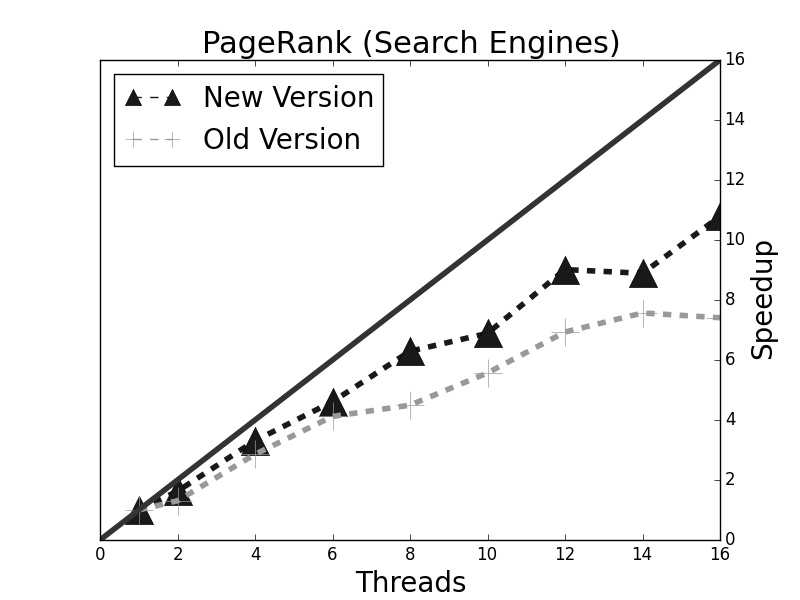
\includegraphics[width=0.3\textwidth]{figures/pagerank-search_engines}}
  \subfloat[]{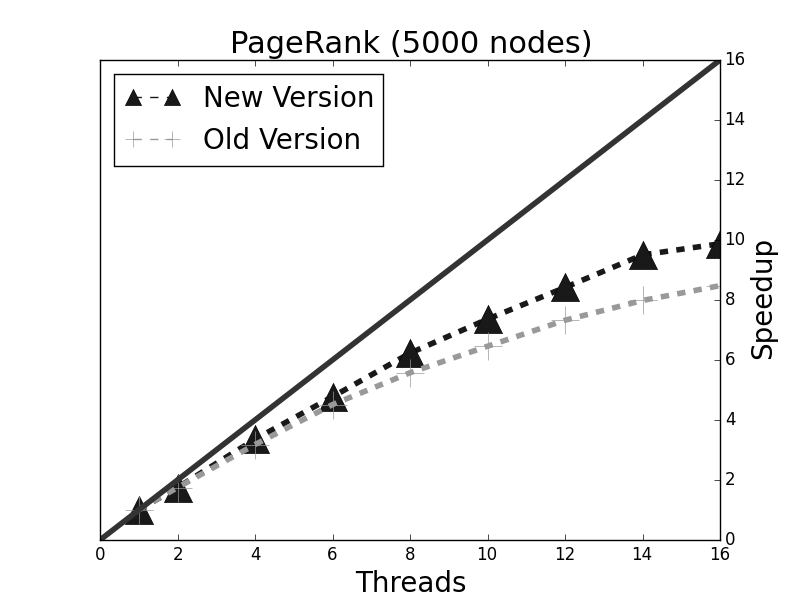
\includegraphics[width=0.3\textwidth]{figures/pagerank-5000}}
  \subfloat[]{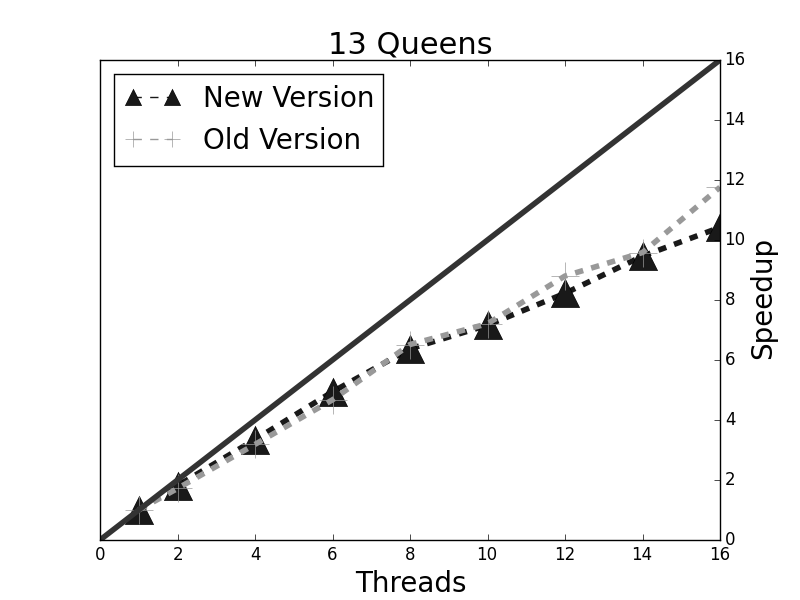
\includegraphics[width=0.3\textwidth]{figures/8queens-13}}
\end{center}
\caption{New experimental results for PageRank and N Queens.}
\label{fig:res1}
\end{figure*}

\begin{figure*}[h]
\begin{center}
  \subfloat[]{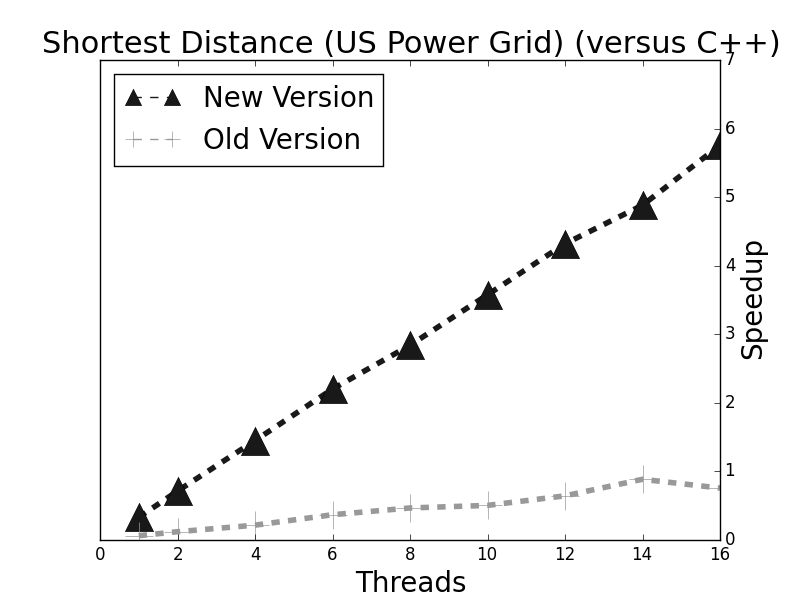
\includegraphics[width=0.3\textwidth]{figures/shortest-uspowergrid}}
  \subfloat[]{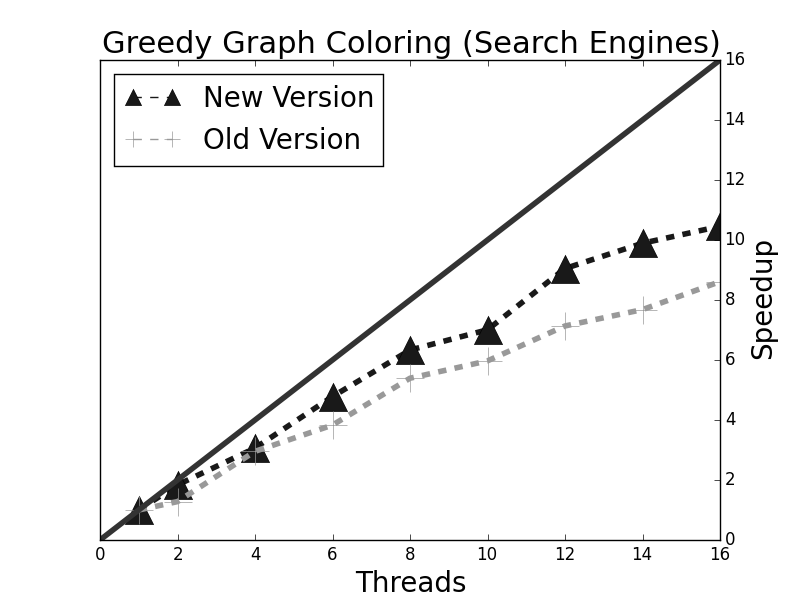
\includegraphics[width=0.3\textwidth]{figures/greedy-graph-coloring-search_engines}}
  \subfloat[]{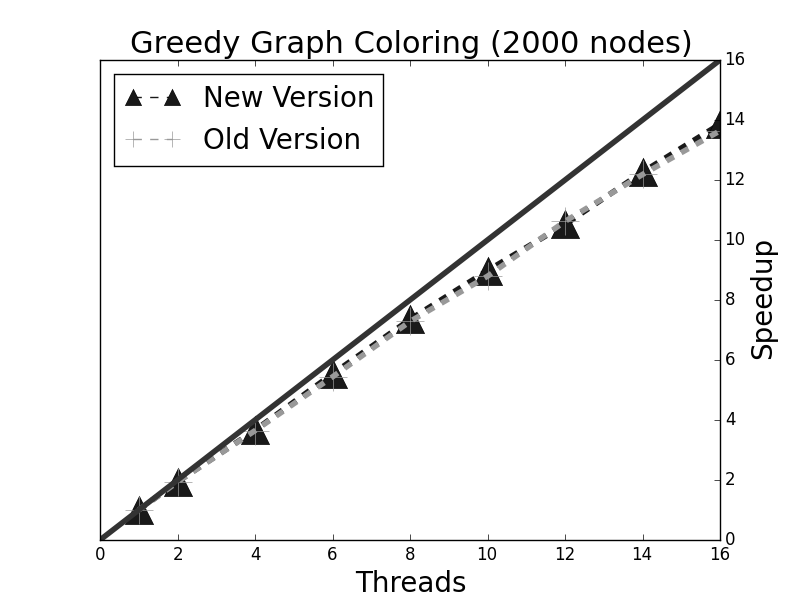
\includegraphics[width=0.3\textwidth]{figures/greedy-graph-coloring-2000}}
\end{center}
\caption{New experimental results for Single Source Shortest Distance and Greedy Graph Coloring.}
\label{fig:res2}
\end{figure*}

\begin{figure*}[h]
\begin{center}
\end{center}
\begin{center}
  \subfloat[]{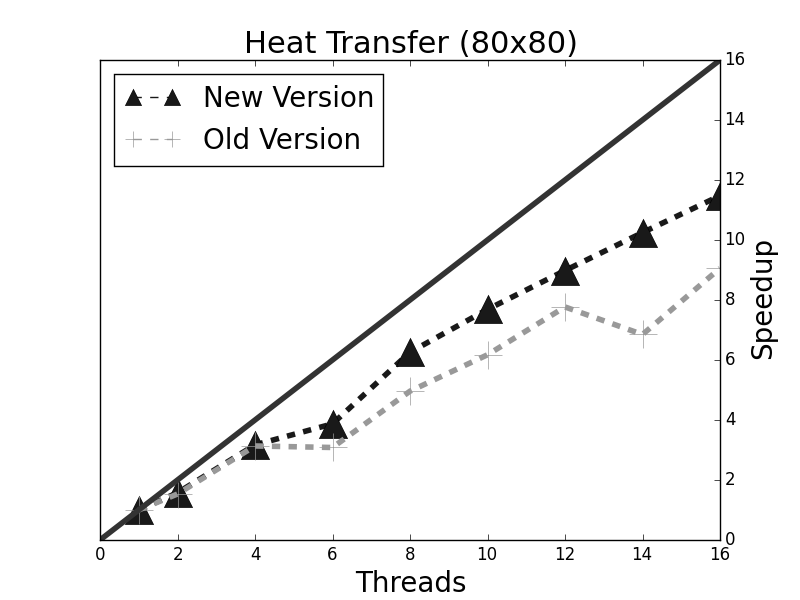
\includegraphics[width=0.3\textwidth]{figures/new-heat-transfer-80}}
  \subfloat[]{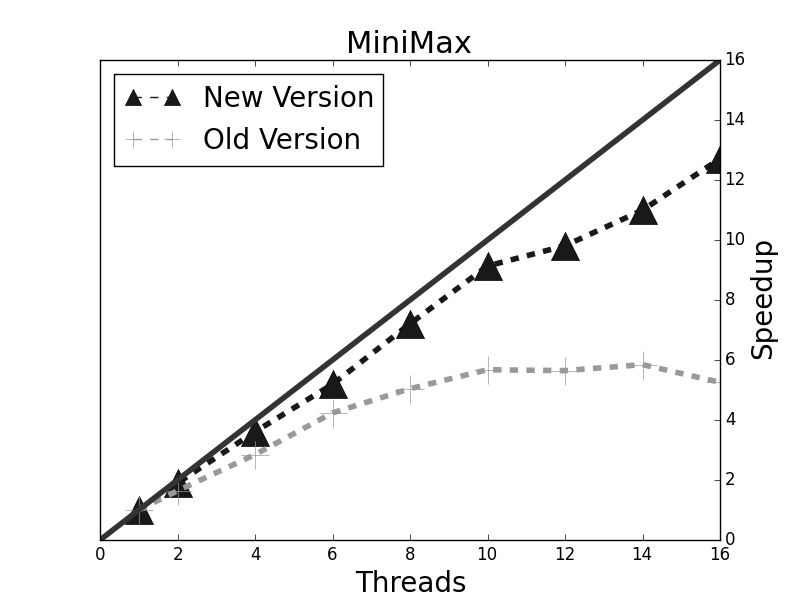
\includegraphics[width=0.3\textwidth]{figures/min-max-tictactoe}}
\end{center}
\caption{New experimental results for Heat Transfer and MiniMax.}
\label{fig:res3}
\end{figure*}

\begin{figure}[b]
\begin{center}
   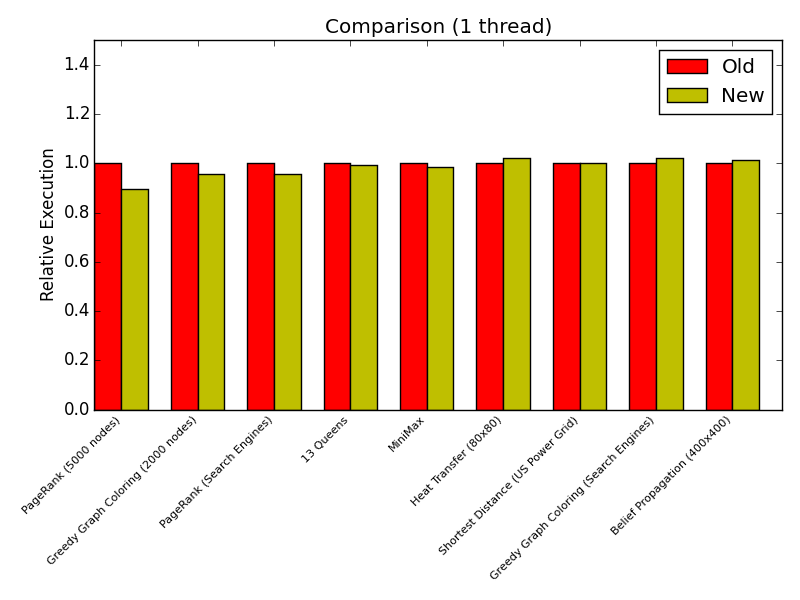
\includegraphics[width=0.9\textwidth]{figures/comparison1}
\end{center}
\caption{Sequential performance of our programs after improving scalability.
   When the "New" value is greater than 1, it means that the new sequential
   execution runs slower than before. Otherwise, values less than 1 mean that it
   now runs faster.}
\label{fig:seq}
\end{figure}

We also measured the impact of our new optimizations when executing the programs
with a single thread. The results presented in Fig.~\ref{fig:seq} indicate
that the sequential execution speed was preserved and some programs even got slightly
faster.

\subsection{Proofs of Interesting Program Properties}

We are mostly focused on proving that our programs compute the intended result.
We have proved informally this property for several programs, including
bipartiteness checking, shortest path, N queens and quick-sort~\footnote{Proofs
available in \url{https://github.com/flavioc/lm-proofs}}.
The proofs reason about the operational semantics of the language and tend to be
relatively short.

\end{document}
